\def\pgfsysdriver{pgfsys-dvipdfm.def}
\documentclass[aspectratio=169]{beamer}
\usetheme[progressbar=foot,titleformat=allcaps,block=fill]{metropolis}
\usepackage{pgfpages}
\pgfmathsetseed{\pdfuniformdeviate 10000000}
\setbeameroption{show notes on second screen}
\setbeamercolor{progress bar}{fg=marigold,bg=marigold!30}%{fg=manitouheights,bg=manitouheights!30}
\setsansfont[BoldFont={Concourse 3 Caps}]{Concourse 3}
%\setsansfont[BoldFont={Heliotrope 3 Caps}]{Heliotrope 3}
%\setmathfont{Fira Math}
%\usepackage{arevmath}
\usepackage[euler-hat-accent]{eulervm}
\setmonofont{Triplicate B Code}
%%% PACKAGES AND INPUTS
\usepackage{pgfopts}
\usepackage{graphicx}
\usepackage{xcolor}
\usepackage{tikz}
\usetikzlibrary{3d,arrows.meta}
\usepackage{verbatim}
\usepackage{comment}
%\input{153controls}
\usepackage{pgfplots}
\usepackage{linalgjh}
\usepackage{amsmath,amssymb,amstext,amsthm,amsfonts}

\usepackage{multicol}


\defaultfontfeatures{Ligatures=TeX}

%%%% LISTINGS

\usepackage{listings}


%%%% COLORS
\definecolor{surfblue}{HTML}{508ac3}
\definecolor{deepblue}{HTML}{243F57}
\definecolor{abyssblue}{RGB}{55,66,84}
\definecolor{marigold}{RGB}{231,147,89}

\definecolor{ash}{HTML}{CBD4C2}
\definecolor{pink-lavender}{HTML}{E0BAD7}
\definecolor{camel}{HTML}{C59F61}

\definecolor{dordtgold}{RGB}{255,184,28}

%%% St. Olaf Colors

%%%% heritage

\definecolor{legacyblack}{RGB}{35,34,34}
\definecolor{manitouheights}{RGB}{216,163,67}

%%%% alternate

\definecolor{heritagegrey}{RGB}{85,87,89}
\definecolor{prairiegrass}{RGB}{239,200,109}

%%%% neutrals

\definecolor{nordicmist}{RGB}{212,224,216}
\definecolor{winterhoarfrost}{RGB}{218,217,214}
\definecolor{cornerstonegrey}{RGB}{189,187,187}

%%%% vibrants

\definecolor{mellbyorange}{RGB}{232,145,68}
\definecolor{chapelcranberry}{RGB}{161,41,87}
\definecolor{norwayvalley}{RGB}{174,212,110}

%%%% brights

\definecolor{wintersunset}{RGB}{214,87,66}
\definecolor{cannonblue}{RGB}{154,216,221}
\definecolor{summersky}{RGB}{43,170,211}

%%%% darks

\definecolor{stainedglass}{RGB}{0,128,125}
\definecolor{olepurple}{RGB}{102,61,91}
\definecolor{hollandnight}{RGB}{42,54,68}

\definecolor{dkgreen}{RGB}{0,0.6,0}
\definecolor{gray}{RGB}{0.5,0.5,0.5}
\definecolor{mauve}{RGB}{0.58,0,0.82}

\setbeamercolor{alerted text}{fg=marigold}%{fg=stainedglass}
\setbeamercolor{normal text}{fg=abyssblue}%{fg=legacyblack}
\setbeamercolor{example text}{fg=surfblue}%{fg=wintersunset}
\setbeamercolor{frametitle}{fg=marigold,bg=black!2}%{fg=manitouheights,bg=black!2}

\definecolor{remgrey}{RGB}{179,179,179}


%%%% MACROS
\def\rem#1{{\hfill \textit{\tiny {\color{remgrey} {#1}}}}}
\def\h#1{\alert{#1}}
\def\C{{\mathbb C}}
\def\Z{{\mathbb Z}}
\def\F{{\mathbb F}}
\def\bF{{\mathbb F}}
\def\Q{{\mathbb Q}}
\def\R{{\mathbb R}}
\def\P{{\mathbb P}}
\def\A{{\mathbb A}}
\def\N{{\mathbb N}}
\def\i{\mathbf i}}
\def\j{\mathbf j}}
\def\k{\mathbf k}}
\def\proj{{\text{proj}}}
\def\comp{{\text{comp}}}
\def\set#1{\left\{ {#1} \right\}}
\def\setof#1#2{{\left\{#1\,:\,#2\right\}}}


%%%% ENVIRONMENTS
\newenvironment{proof-idea}{\noindent{\alert{Proof Idea.}}\hspace*{1em}}{\qed\bigskip\\}
\newtheorem{conj}{Conjecture}
\newtheorem{prop}{Proposition}
\newtheorem{cor}{Corollary}
\newtheorem{defn}{Definition}
\newtheorem{question}{Question}
\newtheorem{goal}{Goal}

\usepackage{cancel}
\newcommand\lheq{\mathrel{\overset{\makebox[0pt]{\mbox{\normalfont\tiny\sffamily \alert{L'H}}}}{=}}}

\title{Welcome to Math 212: Discrete Structures}
%\subtitle{Welcome!}
\author{Dr.\ Mike Janssen}
\date{January 14, 2022}

\begin{document}




%\frame{
%\begin{center}
%		\includegraphics[width=\textwidth]{img/152-02seating.png}
%	\end{center}
%
%}

\frame{\titlepage}

\frame{
	\frametitle{About Dr. Janssen}
	
	\begin{minipage}[c]{0.45\textwidth}
	\begin{itemize}
	\item Year 8 (!!) at Dordt
\item Alma maters: South Dakota (’07), Nebraska (’09, ’13)

\item Enjoys: running, board games, fermentation
\end{itemize}
\end{minipage}
\begin{minipage}[c]{0.45\textwidth}
\begin{center}
		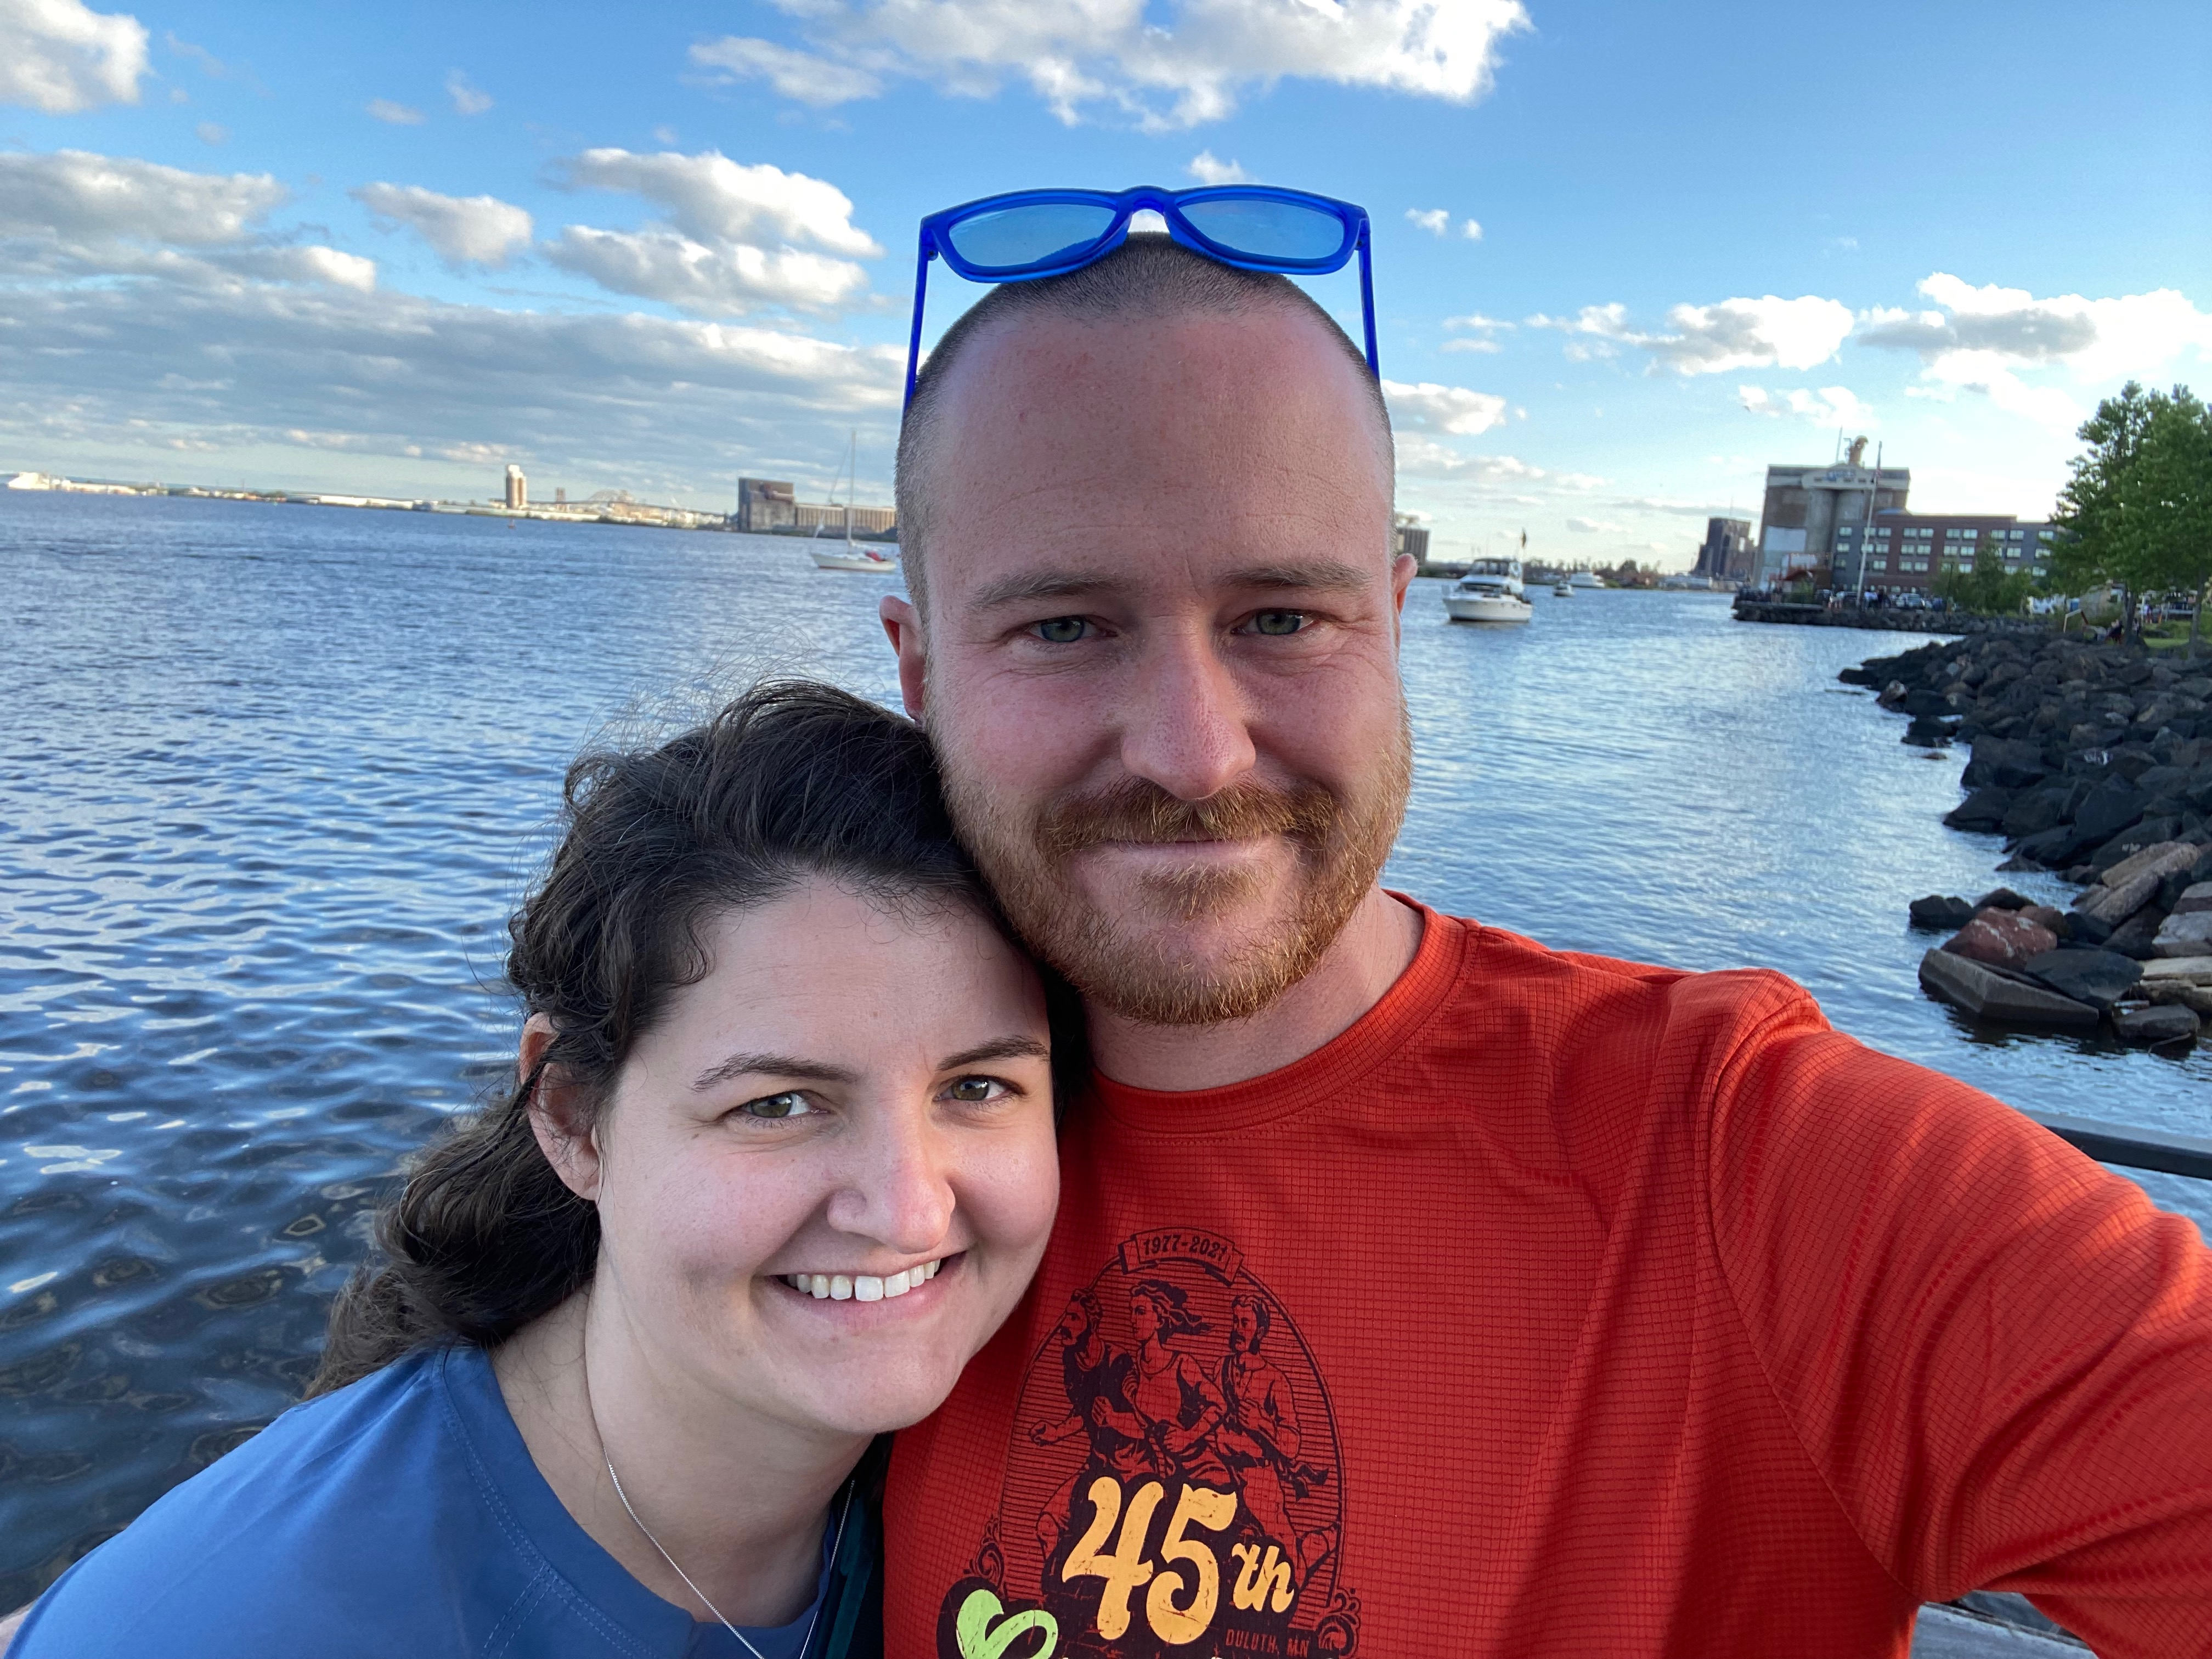
\includegraphics[width=3in]{./img/duluth.jpeg}
	\end{center}
\end{minipage}
	


}

\frame{
	\frametitle{}
	
	\begin{center}
		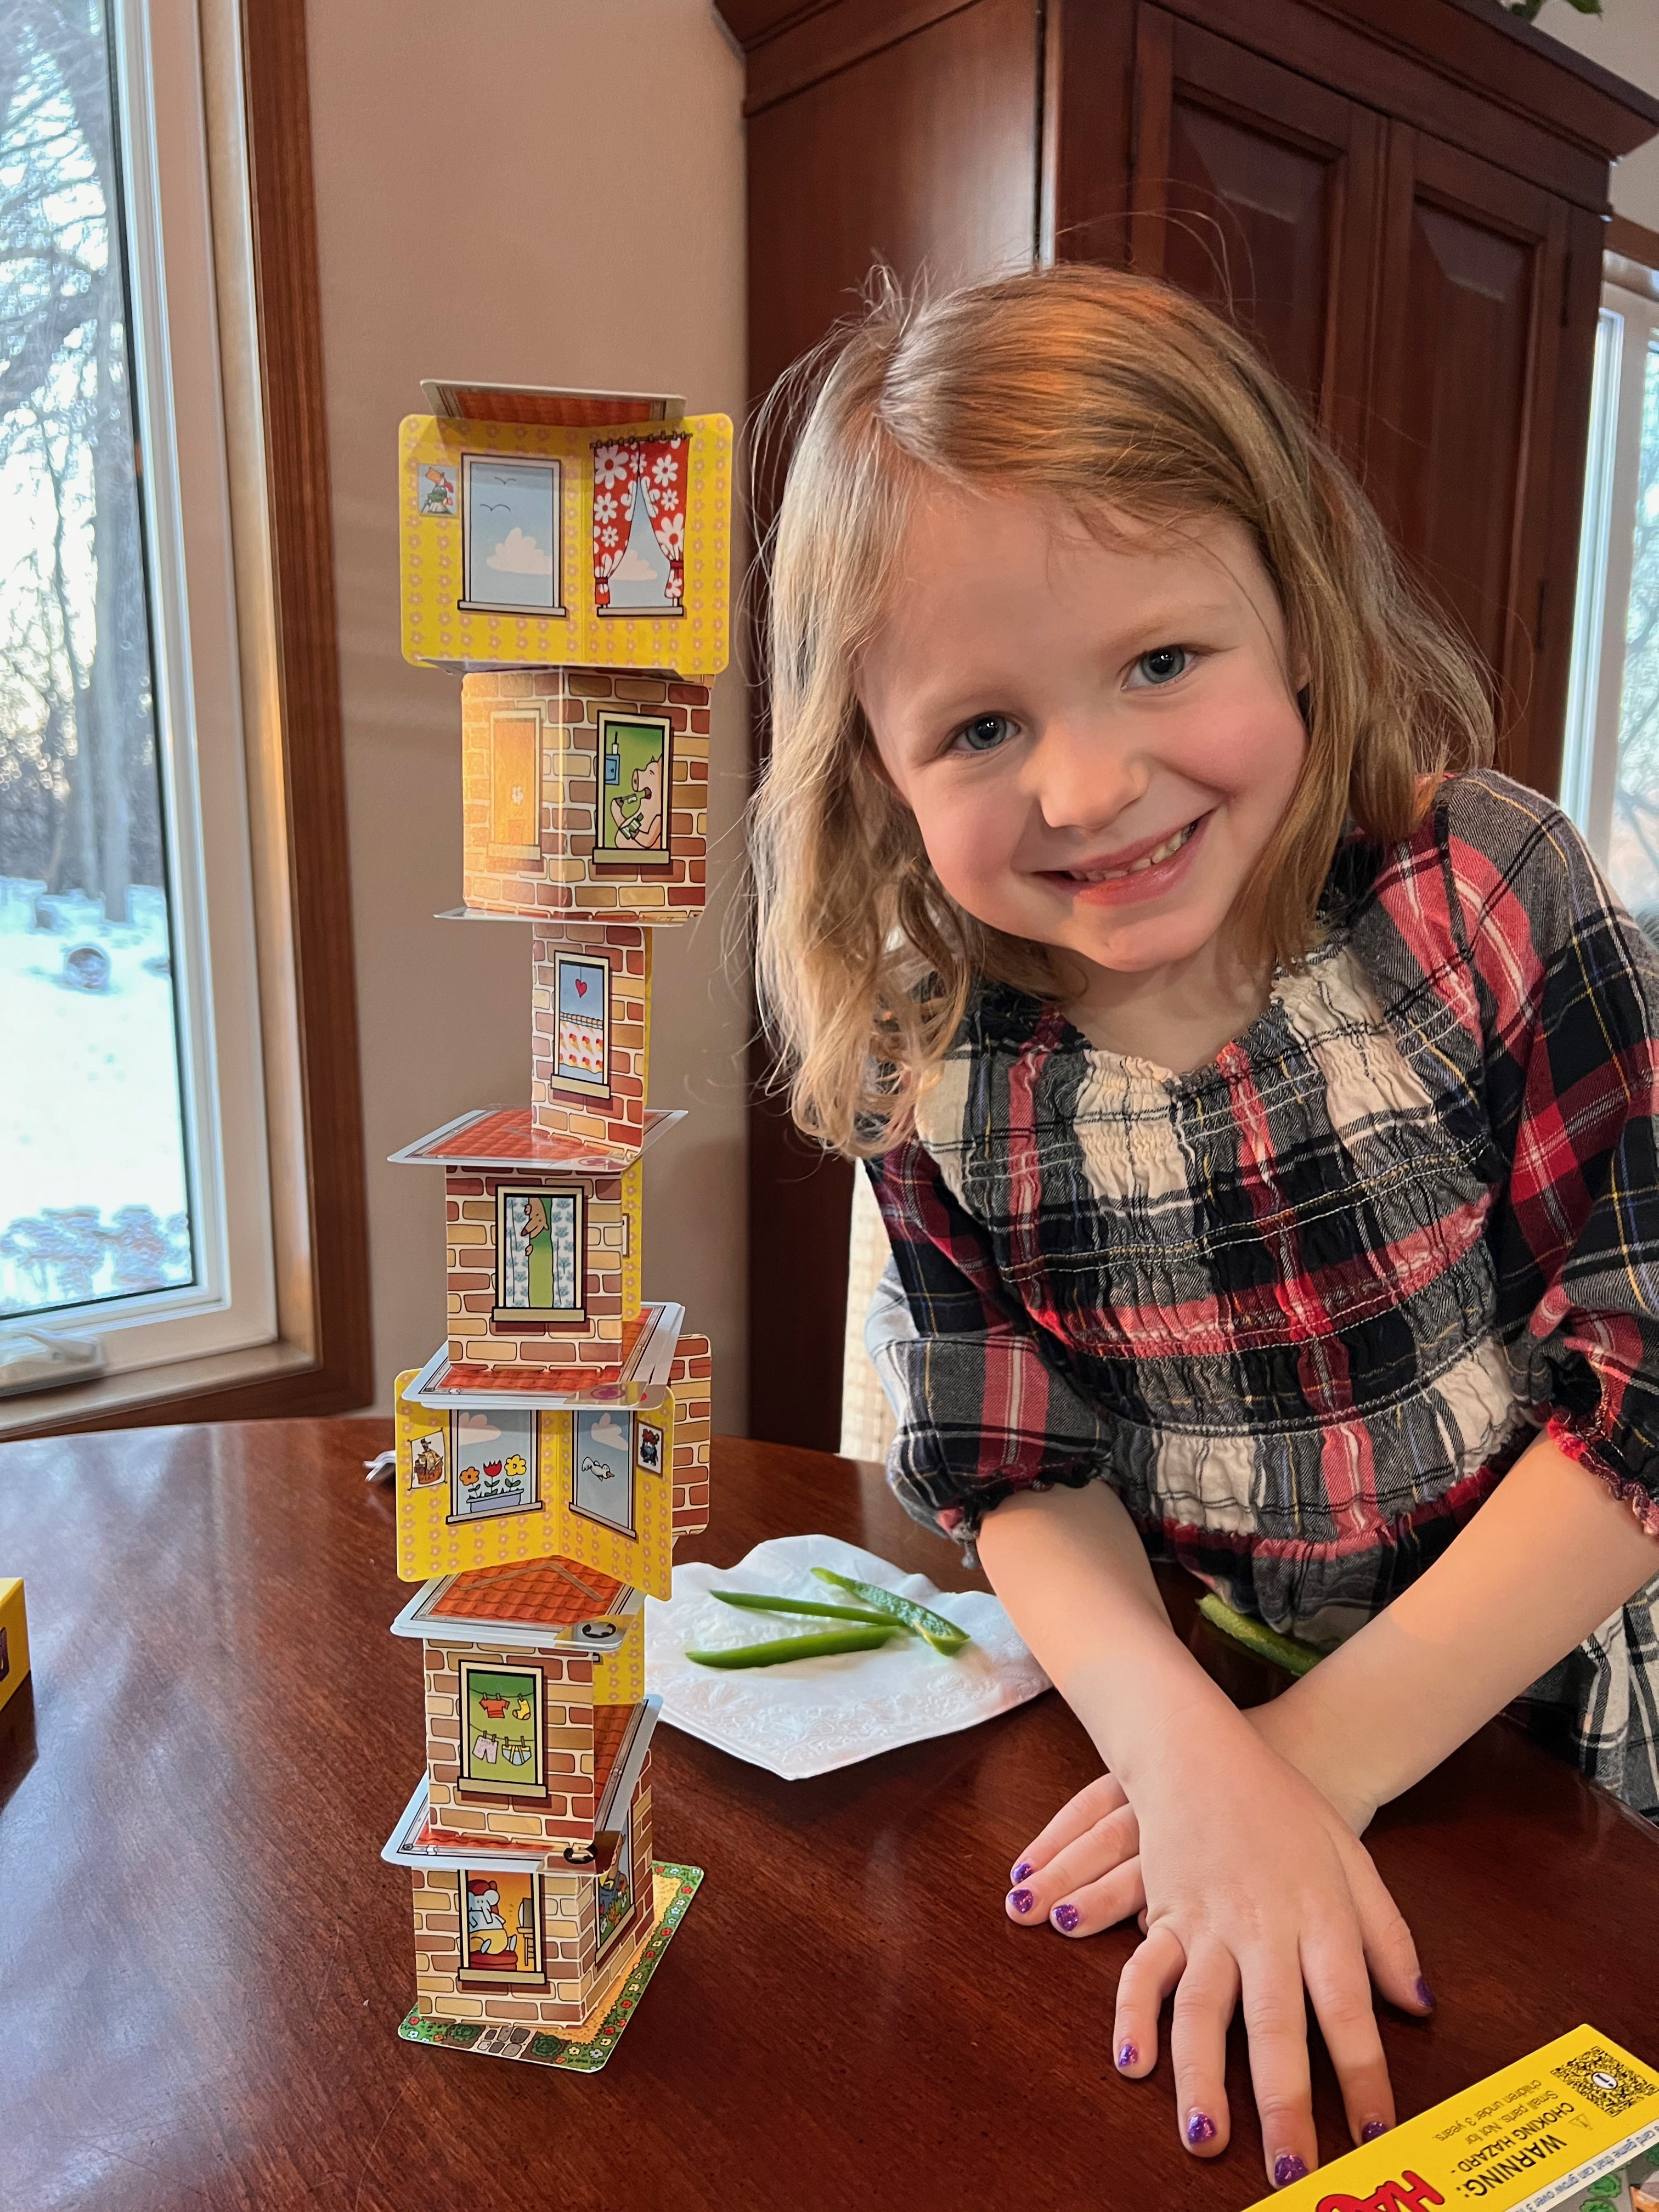
\includegraphics[width=2.5in]{img/lila.jpeg}
		
		Lila (age 5)
	\end{center}

}


\frame{
	\frametitle{}
	
	\begin{center}
		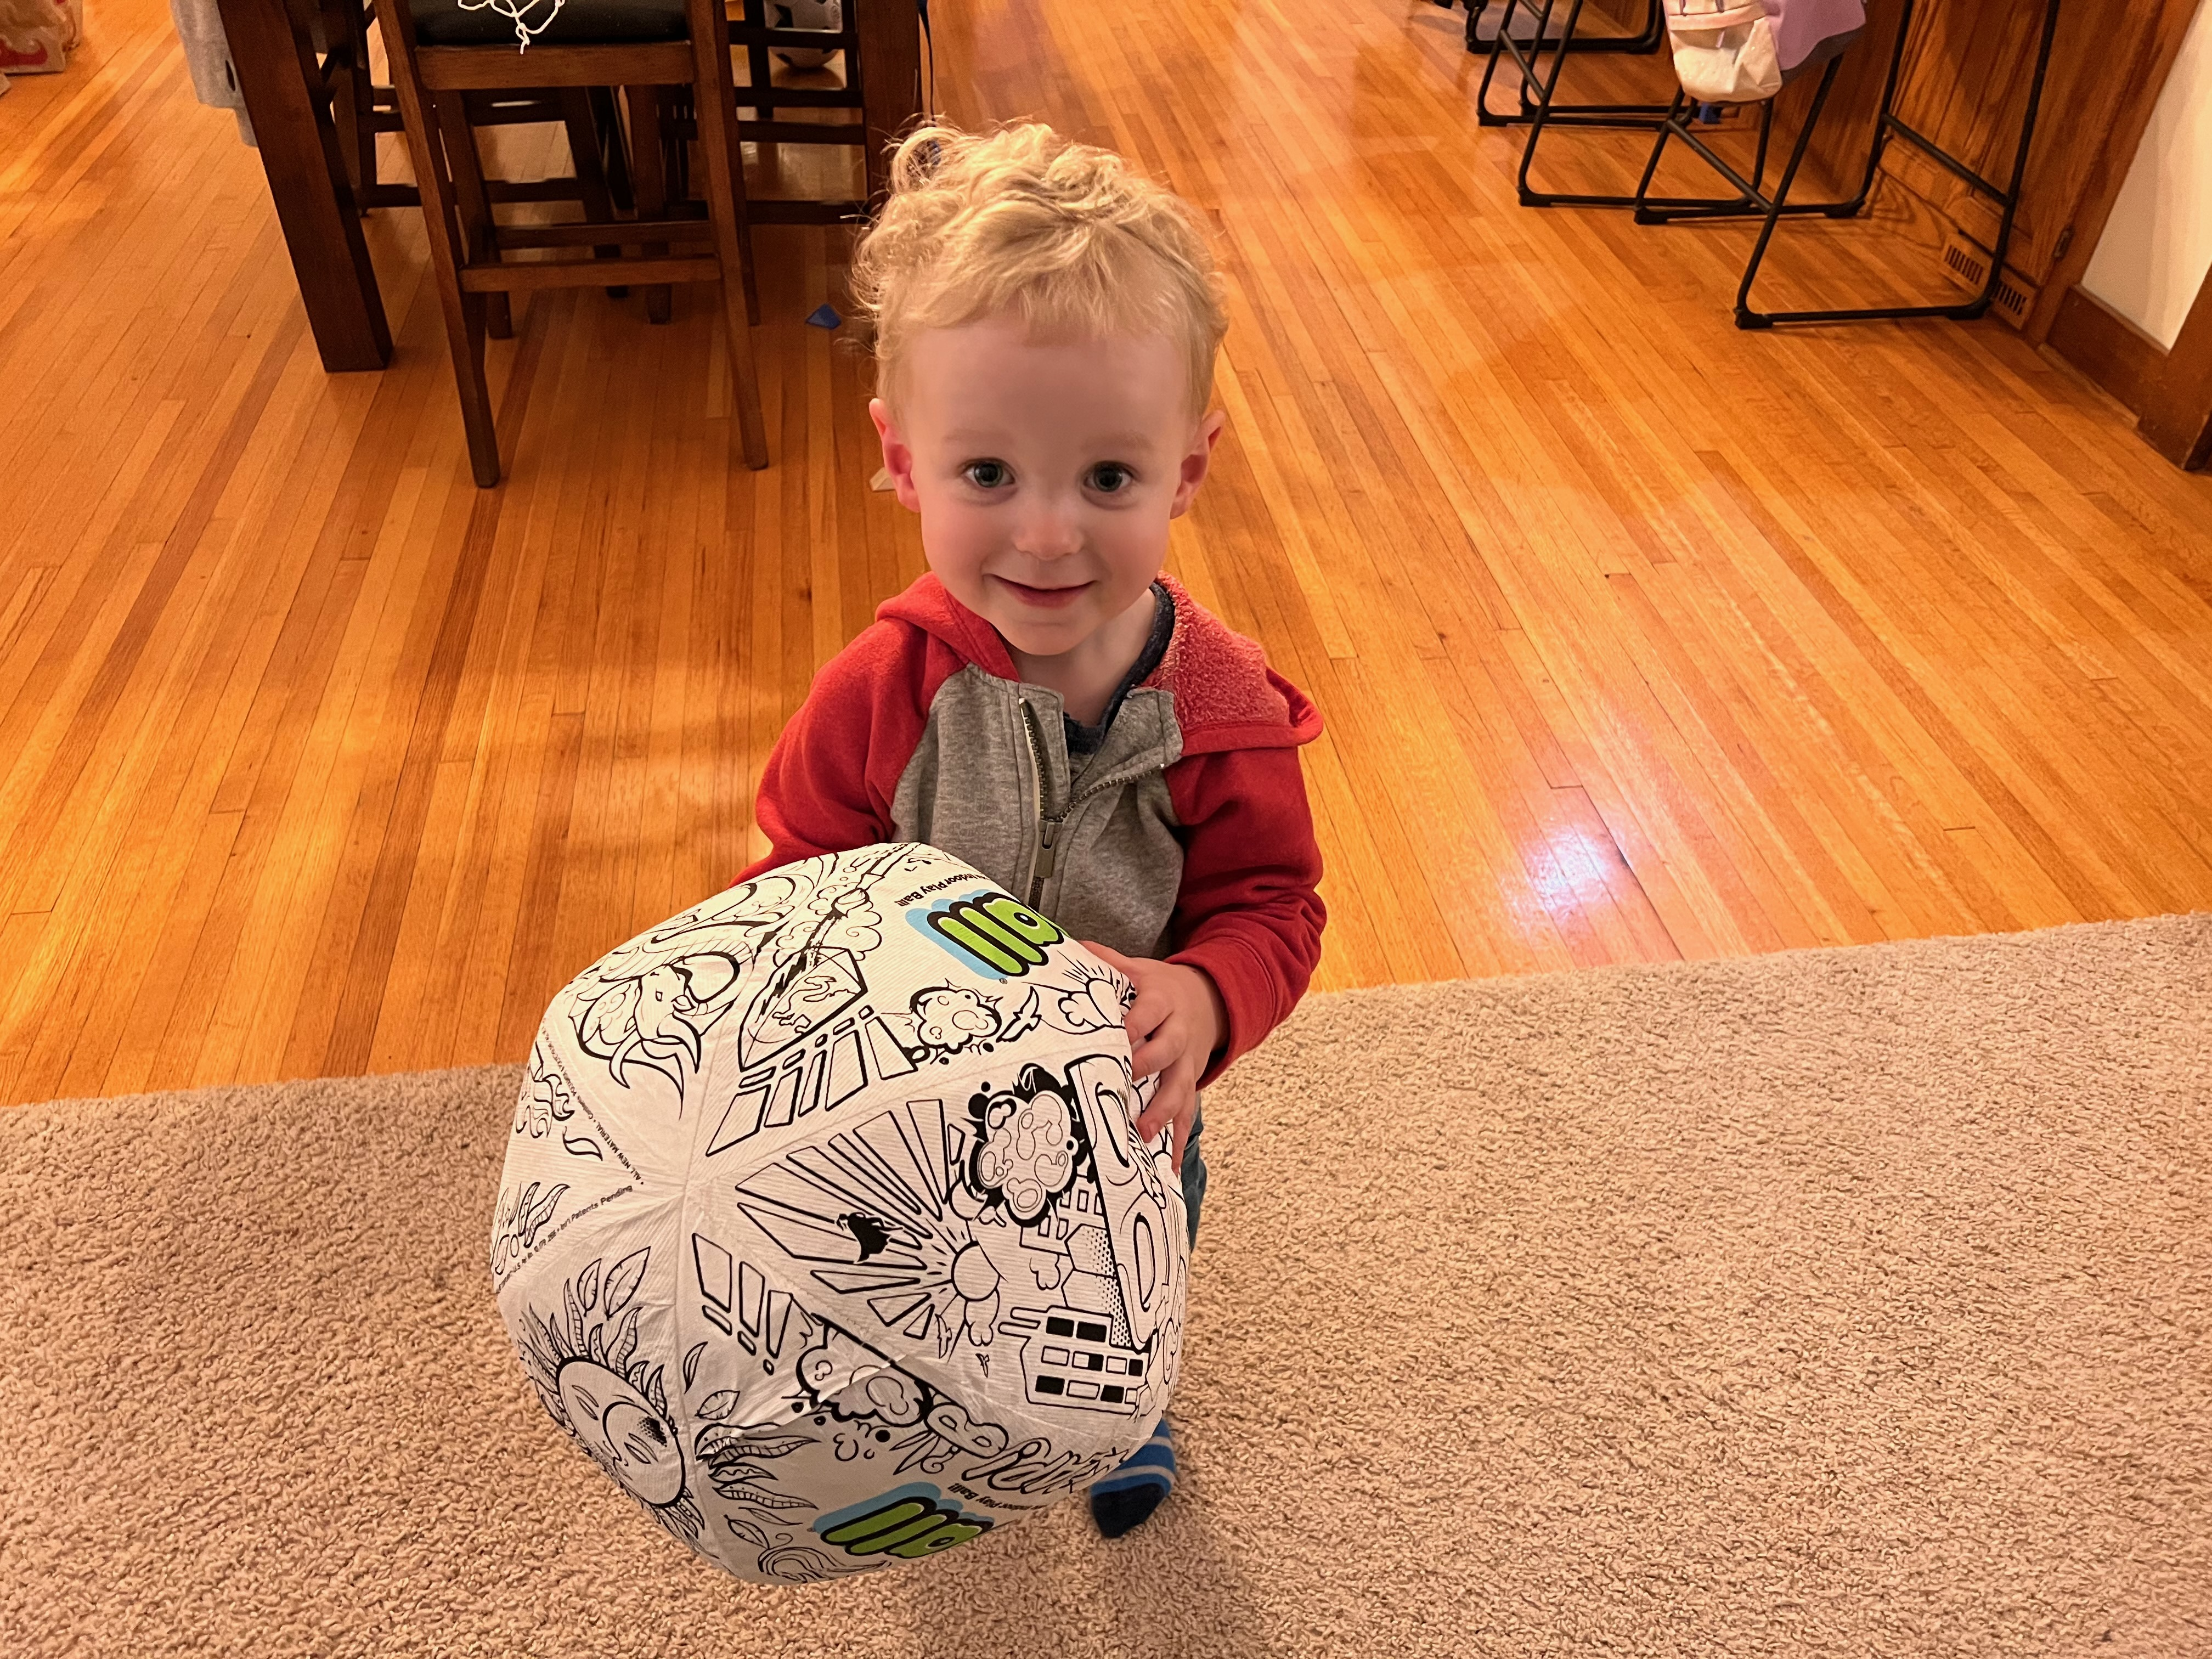
\includegraphics[width=3in]{img/sam.jpeg}
		
		Sam (age 2)
	\end{center}

}



\frame{
	\frametitle{Question 1}
	
	
	\begin{center}
	\Huge
	
	What are the goals of a 
	
	university education?
	
	\end{center}
	


}

\frame{
	\frametitle{Question 2}
	
	
	\begin{center}
	\Huge
	
	How does a person learn something new?
	
	\end{center}
	


}

\frame{
	\frametitle{Question 3}
	
	
	\begin{center}
	\Huge
	
	What do you reasonably expect to remember from your courses in 20 years?
	
	\end{center}
	


}


\frame{
	\frametitle{Question 4}
	
	
	\begin{center}
	\Huge
	
	What is the value of making mistakes in the learning process?
	
	\end{center}
	


}

\frame{
	\frametitle{Claims (via Dana Ernst)}
	
	\begin{itemize}
	\item An education must prepare a student to ask and explore questions in contexts that do not yet exist. That is, we need individuals capable of tackling problems they have never encountered and to ask questions no one has yet thought of.
	\item If we really want students to be independent, inquisitive, and persistent, then we need to provide them with the means to acquire these skills.
\end{itemize}

}


\section{About this course}


\frame{
	\frametitle{Course Liturgies}
	
	
	\begin{itemize}
	\item Pre-class \emph{Daily Work}
	\item In-class presentations by \emph{Presenters} and \emph{Supporters}
	\item \emph{Discussion leaders} and \emph{Scribes} ask questions and write up daily work in a shared document.\pause
	\item Regular \emph{Written Work}, written in \LaTeX--intro due Jan.~19.
	\item Written work graded on an \emph{EMRN} rubric; first one due Jan.~26
	\item Exams (2)
\end{itemize}
	
	

}

\frame{
	\frametitle{a note on the daily work}
	
	\begin{itemize}
	\item No outside resources (books, interent) allowed
	\item OK to ask me questions
	\item Collaboration encouraged, but cite your collaborators
	\item Presentation grade based on \emph{your understanding} and explanations
\end{itemize}

}

\frame{
	\frametitle{Student Hours}
	
	\begin{itemize}
	\item Open Door Policy
	\item Appointments preferred: \texttt{https://calendly.com/mkjanssen/student-hours} (link on Canvas, QR code outside my door)
	\item Masks required in student hours through the end of the month; reevaluate in February
\end{itemize}

}


\frame{
	\frametitle{Advertisement}
	
	\begin{itemize}
	\item Get paid to do summer research in mathematics at Dordt!
	\item Tentative dates: June 6-July 29
	\item Success in this class would prepare you well
	\item Applications due at the end of the month
	\item Ask me if you have any questions
\end{itemize}

}

\frame{
	\frametitle{Daily Work Assignment 1}
	
	Head to 
	
	\begin{center}
	\texttt{notes.mkjanssen.org/ds}
	\end{center}
	
	And work on Activities/Problems
	
	\begin{itemize}
	\item 1.1.2
	\item 1.1.3
	\item 1.2.4
	\item 1.2.11
	\item 1.2.12.
\end{itemize}
	 

}







\end{document}